\documentclass[12pt, a4paper]{report}
\usepackage[utf8]{inputenc}
\usepackage{lscape}   % Make a page in landscape format \begin{landscape}
\usepackage{colortbl} % To color table cells
\usepackage{color} % Able to change textcolor
\usepackage[table]{xcolor}
\usepackage{longtable}
\usepackage{graphicx} % Able to add pictures
\usepackage{parskip}  % Separate paragraphs with a blank line
                      % rather than using indentation
\usepackage{hyperref} % Support for hyperlinks
\usepackage[protrusion=true,expansion=true]{microtype} % Improve justification
\usepackage{subfigure}
\usepackage{hyperref}
\usepackage{caption}
\usepackage{float}

\usepackage{lipsum}
\usepackage{wrapfig}
\usepackage{array}
\usepackage{sidecap}
\usepackage{appendix}
\usepackage{fancyhdr}
\usepackage{changepage}
\usepackage[margin=1.3in]{geometry}
\usepackage{amsmath}
\usepackage{enumitem}
\usepackage{pdflscape}
\usepackage{afterpage}
\usepackage{longtable}


\newcommand{\gray}{\rowcolor[gray]{.90}}

\hypersetup{%
    pdfborder = {0 0 0}
}

\begin{document}
	\begin{titlepage}
\begin{center}

{\Huge \bf Compendium} \\[1.0cm]
{\Huge \bf TDT4242} \\[1.0cm]
{\Large \bf Requirements and Testing} \\[1.0cm]
\vspace{1cm}

{\bf By Marte Løge}


\end{center}
\end{titlepage}
	\clearpage
	\tableofcontents
	\clearpage
	\chapter{Use case}

We chose to make use cases, both diagrams and textual, in the standard UML notation. 
The use cases will help us in many ways; it will improve the communication about the 
system in the group, as well as making a common agreement about the system requirements.

The use cases can also be a good tool when making tests, the “Description”, “Data”, 
“Flow of events”, and the “Response” fields in the use cases can easily be 
transferred over to the tests. The use cases can also be a good measure of the gap 
between the requirements and the developed software, when we are deciding whether to 
ship or not to ship the system.

The use cases are based on the scenarios from the SoCam documentation paper. 


\clearpage

\section{Scenario 1}

	\begin{figure}[H]
		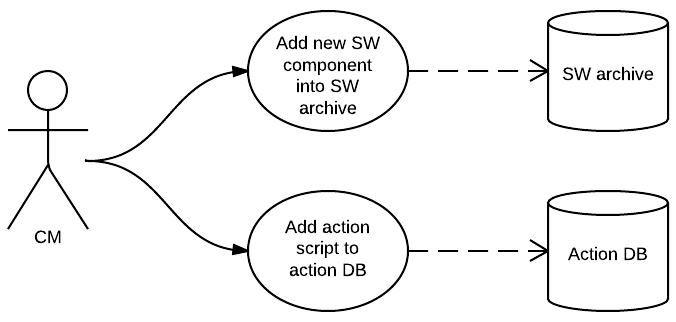
\includegraphics[width=\textwidth]{pics/usecase1.png}
	\end{figure}

	\begin{table}[H]
		\begin{tabular}{ p{4cm} | p{10cm} }
			\hline
			\rowcolor{gray}
			{\bf Use case} & {\bf A new version of a software component} \\ \hline
			{\bf Actors} & CM - Configuration team\\ \hline
			{\bf Application} & Socam \\ \hline
			{\bf Description} & A CM responsible wants to add a new SW-component to the 
			SW archive, the person also have to update the Action DB with the actionscript 
			that connects the SW-component to the ECU.\\ \hline
			{\bf Preconditions} & {\bf 1)} Running computer {\bf 2)} Log on to the system {\bf 3)} ECU already in system\\ \hline
			{\bf Data} & SW + actionscript \\ \hline
			{\bf Stimulus} & A new software component is created by the SW department \\ \hline
			{\bf Flow of events} & 

				\begin{enumerate}[font=\bfseries]
					\item CM enters the new SW component to the system and uploads it to the SW archive
					\begin{enumerate}[label*=\arabic*., font=\bfseries]
						\item CM enters invalid component. 
					\end{enumerate}
					
					\item CM adds the new actionscript and uploads it to the Action DB
					\begin{enumerate}[label*=\arabic*., font=\bfseries]
						\item CM enters invalid actionscript
					\end{enumerate}
				\end{enumerate}
			
			\\ \hline
			{\bf Response} & Both the new SW component and actionscript are 
			successfully uploaded to the respective databases \\ \hline

		\end{tabular}
	\end{table}

\section{Scenario 2}

	\begin{figure}[H]
		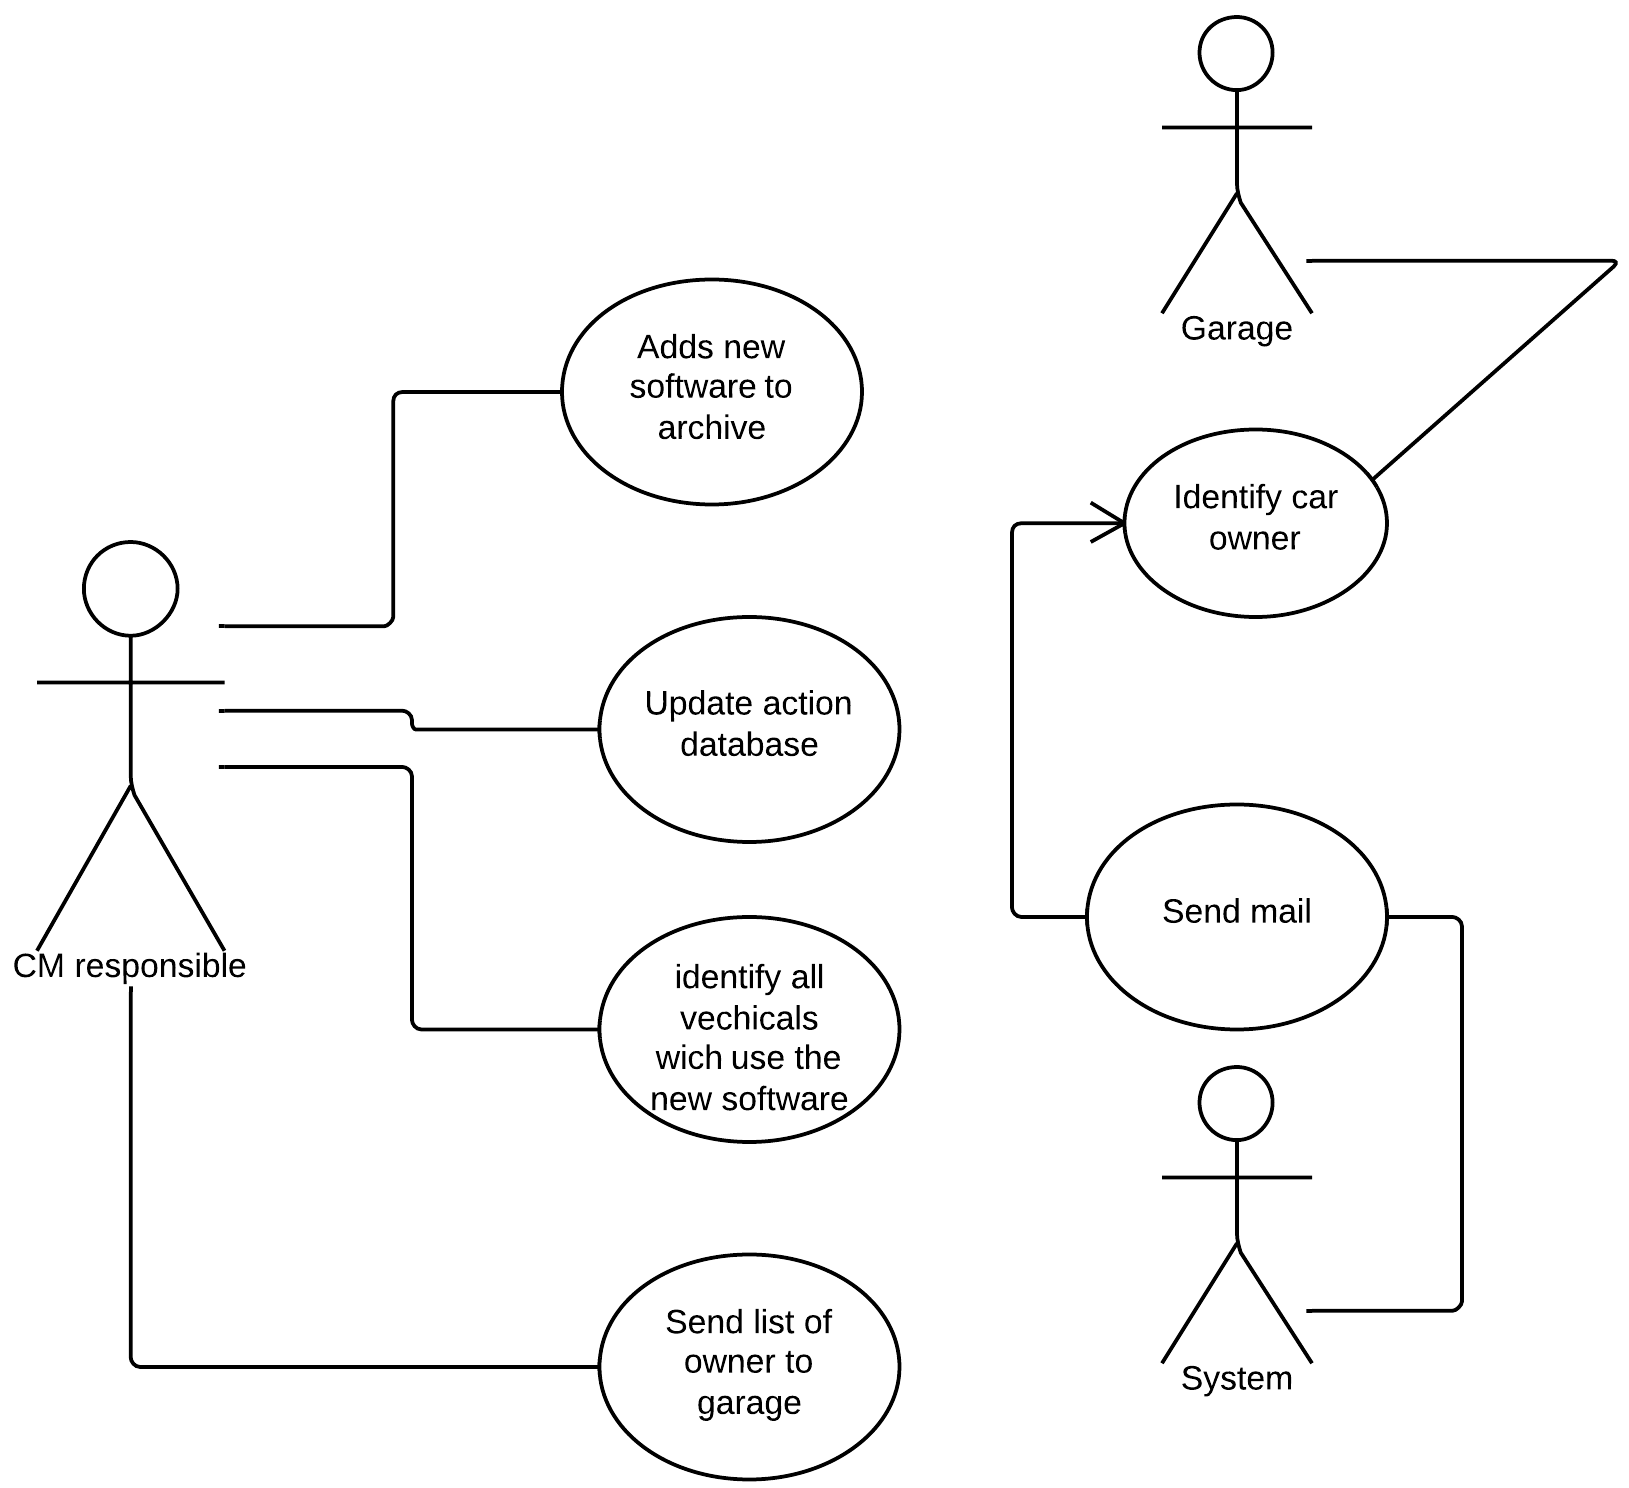
\includegraphics[width=\textwidth]{pics/usecase2.png}
	\end{figure}

	\begin{table}[H]
		\begin{tabular}{ p{4cm} | p{10cm} }
			\hline
			\rowcolor{gray}
			{\bf Use case} & {\bf A safety critical software defect is discovered} \\ \hline
			{\bf Actors} & CM responsible, System, Garage \\ \hline
			{\bf Application} & Socam \\ \hline
			{\bf Description} & When a safety critical software defect is discovered a CM 
			responsible will repair the defect and make it availabel in the database. 
			The garage will then make sure that all the relevant carowners get information 
			about the defect and the system improvments.\\ \hline
			{\bf Preconditions} & {\bf 1)} Running computer {\bf 2)} Log on to the system \\ \hline
			{\bf Data} & SW + actionscript \\ \hline
			{\bf Stimulus} & New software is developed \\ \hline
			{\bf Flow of events} & 
				\begin{enumerate}[font=\bfseries]
					\item add new software to the archive
						\begin{enumerate}[label*=\arabic*., font=\bfseries]
							\item The software allready exist 
						\end{enumerate}
					\item update actionscript database
						\begin{enumerate}[label*=\arabic*., font=\bfseries]
							\item Connection to database fails. 
						\end{enumerate}
					\item Identify all vehicles that will be using the new system.
					\item CM responsible logs out
					\item List of vehicles is send to all registered garage.
						\begin{enumerate}[label*=\arabic*., font=\bfseries]
							\item  List of vehicles is not received by the garage.
						\end{enumerate}
					\item Garage employee identifies relevant car owners.
						\begin{enumerate}[label*=\arabic*., font=\bfseries]
							\item Car has no registered owner.
						\end{enumerate}
					\item System makes e-mail that is send to all the car owners.
						\begin{enumerate}[label*=\arabic*., font=\bfseries]
							\item Sending e-mail fails.
						\end{enumerate}
				\end{enumerate}
			
			\\ \hline
			{\bf Response} &  \\ \hline
		\end{tabular}
	\end{table}

\clearpage

\section{Scenario 3}
	
	\begin{figure}[H]
		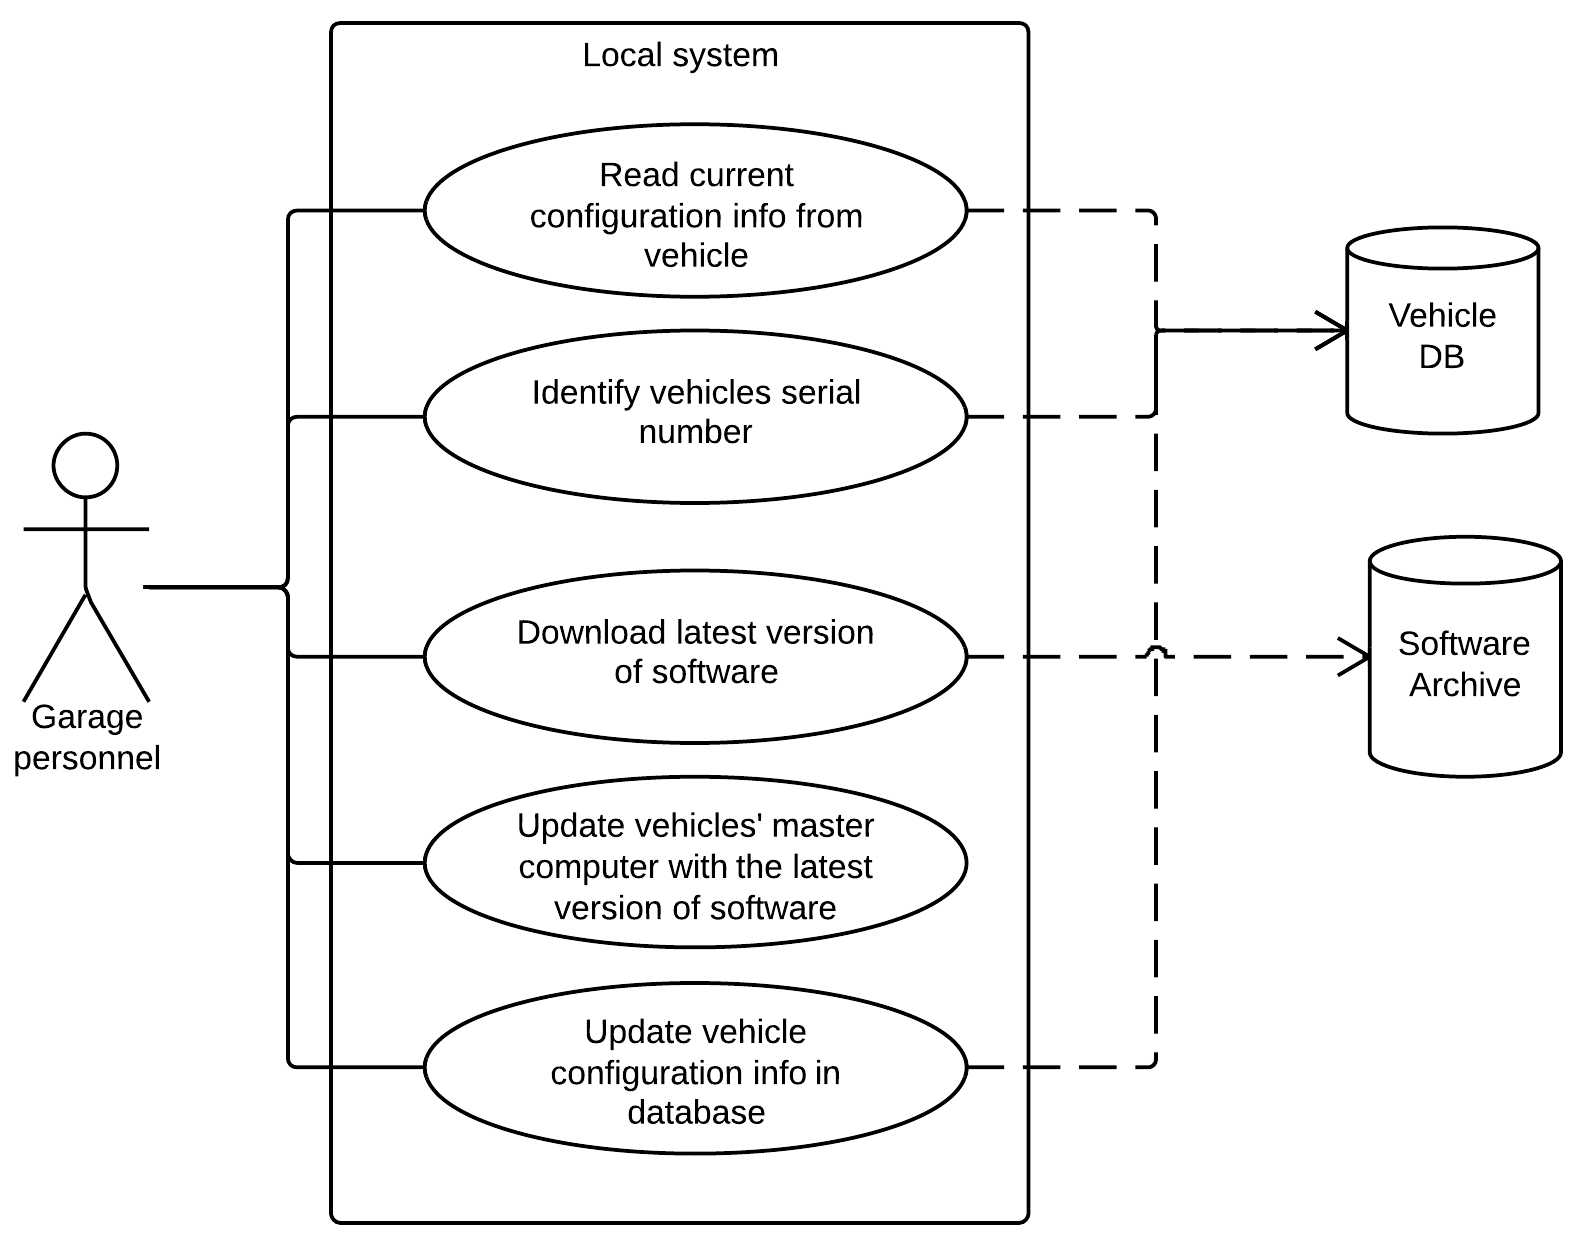
\includegraphics[width=\textwidth]{pics/usecase3.png}
	\end{figure}

		\begin{table}[H]
		\begin{tabular}{ p{4cm} | p{10cm} }
			\hline
			\rowcolor{gray}
			{\bf Use case} & {\bf A vehicle is scheduled for maintanance} \\ \hline
			{\bf Actors} & Garage personnel\\ \hline
			{\bf Application} & Socam \\ \hline
			{\bf Description} & A vehicle is scheduled for maintenance. The vehicle 
			is controlled and updated with the latest version of software. \\ \hline
			{\bf Preconditions} & \\ \hline
			{\bf Data} & Vehicle configuration info, vehicle serial number, software update \\ \hline
			{\bf Stimulus} & A vehicle is scheduled for maintainance \\ \hline
			{\bf Flow of events} & 
				\begin{enumerate}[font=\bfseries]
					\item Read the current configuration info from the vehicle
					\item The garage personnel identifies the vehicles serial 
					number from the owners name.
					\item Downloads the latest version of software 
						\begin{enumerate}[label*=\arabic*., font=\bfseries]
							\item The car is already up to date with the latest software, jump to 6.
						\end{enumerate}
					\item Updates the vehicles master computer with the latest software.
					\item The database is updates with vehicles software updates
					\item Finished
				\end{enumerate}
			
			\\ \hline
			{\bf Response} & Software update successful  \\ \hline

		\end{tabular}
	\end{table}


\clearpage
\section{Scenario 4}

	\begin{figure}[H]
		\centering
		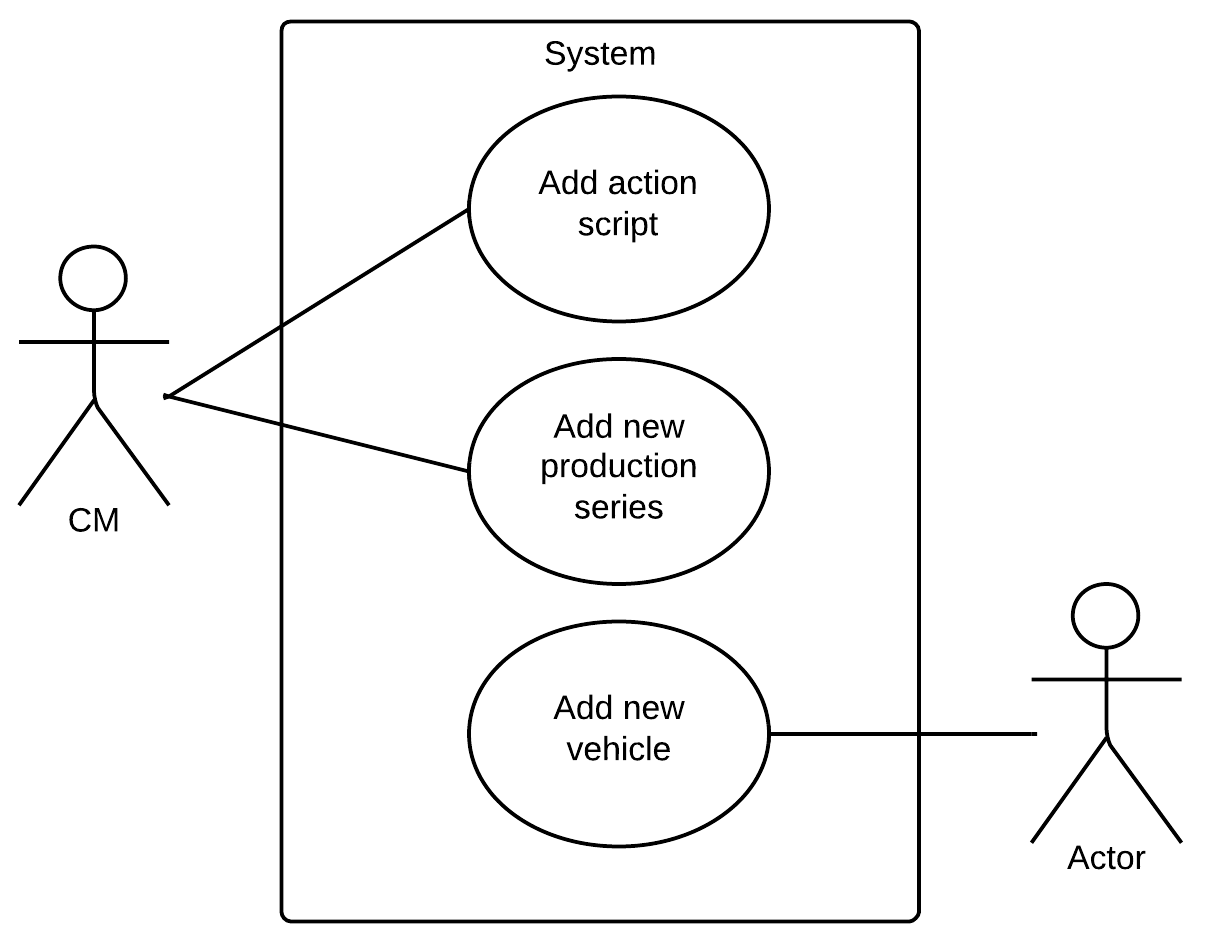
\includegraphics[scale=0.25]{pics/usecase4.png}
	\end{figure}


	\begin{table}[H]
		\centering
		\begin{tabular}{  p{4cm} | p{10cm} }
			\hline
			\rowcolor{gray}
			{\bf Use case} & {\bf A new vehicle is finished from the factory} \\ \hline
			{\bf Actors} & CM - Configuration team, FP - Factory personel \\ \hline
			{\bf Application} & Socam \\ \hline
			{\bf Description} & A new series of vehicle is made and needs to be 
			added into the system \\ \hline
			{\bf Preconditions} & {\bf 1)} Running computer {\bf 2)} Log on to the system \\ \hline
			{\bf Data} & Vehicle series information and specific vehicle \\ \hline
			{\bf Stimulus} & A new vehicle series is added into the system \\ \hline
			{\bf Flow of events} & 
				\begin{enumerate}[font=\bfseries]
					\item CM adds a new action script to the action script database
						\begin{enumerate}[label*=\arabic*., font=\bfseries]
							\item Not valid action script
							\item Not valid parameters given when adding a new vehicle 
							production serie.
							\item Not valid parameters given when adding a new vehicle 
							to the database
							\item Action script is saved with errors
						\end{enumerate}
					\item CM adds the new serie of vehicle to the vehicle database
					\item FP adds a new vehicle to a vehicle production series in the vehicle database. 
				\end{enumerate}
			
			\\ \hline
			{\bf Response} & Confirmation that product has been registered. \\ \hline
		\end{tabular}
	\end{table}
	\clearpage
	\chapter{Risk Assessment}

	The risk assesment table is our base criteria for total risk assessment. The table tells 
	the risk of different combinations of consequence and probability. The consequence and 
	probability is ranked High, Medium and Low. 

		\begin{figure}[H]
			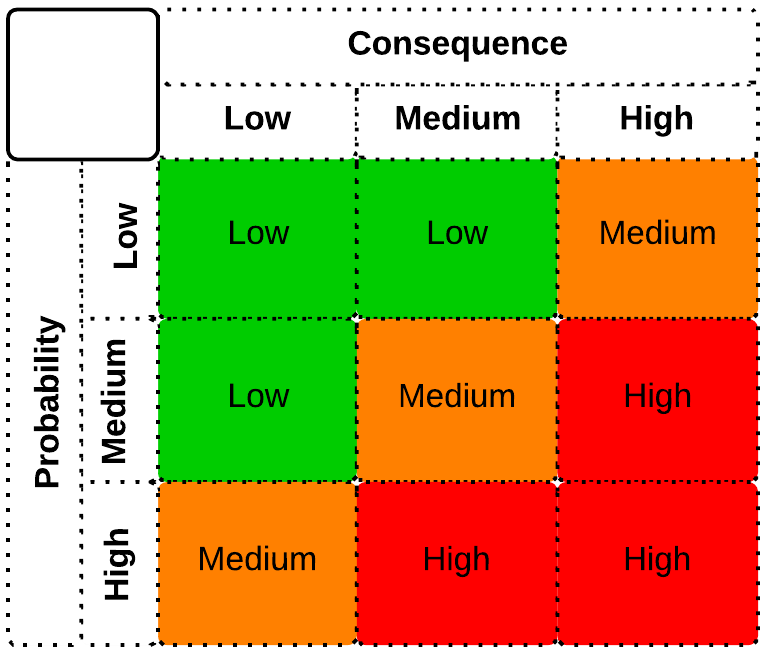
\includegraphics[scale=0.3]{pics/risk.png}
		\end{figure}

	In the following tables we have performed a risk identification and a risk assessment for 
	each separate use case. In the risk identification we have evaluated each function and 
	considered what may go wrong. In addition we have evaluated where in the source code the 
	error may occur. For each use case and risk assessment, we have rated the risk for the customer, 
	the user and the developer. 

	\clearpage


	\begin{landscape}

	\section{Scenario 1}
			\begin{longtable}{ c | p{5cm} | p{5cm} | p{5cm} | c | c | c}
				\hline
				{\bf ID} & {\bf Function} & {\bf Failure mode} & {\bf Code involved} & 
				{\bf Cons.} & {\bf Prob.} & {\bf Tot.} \\ \hline
				1.1 
				& CM enters the new SW component to the system and uploads it to the SW archive
				& CM enters invalid component & FactoryProjectPane, FactoryProject
				& High & Med & High \\ \hline
				1.2 
				& CM adds the new actionscript and uploads it to the Action DB
				& CM enters invalid actionscript
				& FactoryProjectPane, FactoryProject 
				& High & Med & High \\ \hline
		\end{longtable}	

	\section{Scenario 2}

			\begin{longtable}{ c | p{5cm} | p{5cm} | p{5cm} | c | c | c}
				\hline
				{\bf ID} & {\bf Function} & {\bf Failure mode} & {\bf Code involved} & 
				{\bf Cons.} & {\bf Prob.} & {\bf Tot.} \\ \hline
				2.1 
				& CM adds new software to the archive
				& The software already exist. 
				& FactoryProjectPanel, FactoryProject, FactoryDBStorage, SoftwarePanel, Software
				& Low & Low & Low \\ \hline
				2.2 
				& CM update actionscript database
				& Invalid actionscript
				& FactoryDBStorage, CreateFactoryDB
				& High & Med & High \\ \hline
				2.3
				& List of vehicles is send to all registered garage.
				& The garage do not receive the list.
				& FactoryProjectPanel, RecallPanell
				& High & Med & High \\ \hline
				2.4
				& Garage employee identifies relevant car owners.
				& The car has no registered owner
				& ProjectPanel, RecallPanel, PersonPanel, PersonListModel
				& Med & Low & Low \\ \hline
				2.5
				& System sends email to all relevant car owners.
				& Email is not sendt, Sendt email is not received
				& ProjectPanel, RecallPanel, PersonPanel
				& Med & Med & Med \\ \hline
			
		\end{longtable}

	\section{Scenario 3}

		\begin{table}[H]
			\begin{tabular}{ c | p{5cm} | p{5cm} | p{5cm} | c | c | c}
				\hline
				{\bf ID} & {\bf Function} & {\bf Failure mode} & {\bf Code involved} & 
				{\bf Cons.} & {\bf Prob.} & {\bf Tot.} \\ \hline
				3.1 
				& GP identifies the vehicle serial number
				based on the RO's name.  
				& No match on the RO's name in the databse
				& ProjectPanel, SearchPersonAction 
				& Low & Med & Med \\ \hline
				3.2
				& GP downloads the latest version of software
				from the software archive 
				& Could not find the lastest version of software
				in the software archive.
				& ProjectPanel, VehiclePanel, Vehicle, VehicleDBStorage, GUIConnect, garageConnection
				& Med & Low & Low \\ \hline
				3.3 
				& GP updates the vehicles master computer with
				the latest version of software from the Software
				archive 
				& The vehicle is already updated with the latest
				software version.
				& ProjectPanel, Connection, GUIConnect, 
				VehiclePanel, Vehicle
				& Low & Low & Low \\ \hline
				3.4 
				& GP updates the vehicles configuration info 
				in the vehicle DB. 
				& The configuration info was not updated.
				& ProjectPanel, VehiclePanel, 
				Vehicle
				& Med & Med & Med \\ \hline
			\end{tabular}
		\end{table}


	\section{Scenario 4}

		\begin{table}[H]
			\begin{tabular}{ c | p{5cm} | p{5cm} | p{5cm} | c | c | c}
				\hline
				{\bf ID} & {\bf Function} & {\bf Failure mode} & {\bf Code involved} & 
				{\bf Cons.} & {\bf Prob.} & {\bf Tot.} \\ \hline
				4.1
				& CM adds a new actionscript to the action database
				& CM adds a invalid action script
				& FactoryProjectPanel, EcuVehPanel, Ecu, Software, SimpleEcu, EcuDbStorage
				SoftwareDbStorage
				& High & Med & High \\ \hline
				4.2
				& CM adds the new serie of vehicle to the vehicle database
				& Parameters given when adding the new series is not valid
				& FactoryProjectPanel, NewVehiclePanel, Vehicle, VehicleDBStorage
				& Med & Low & Low \\ \hline
				4.3
				& FP adds a new vehicle to the vehicle production series in the vehicle database
				& Parameters given when adding the new vehicle is not valid
				& FactoryProjectPanel, NewVehiclePanel, Vehicle, VehicleDBStorage
				& Low & Med & Low \\ \hline

			\end{tabular}
		\end{table}


\end{landscape}
	\clearpage
	\chapter{Test Strategy}

	\clearpage

	{\bf What’s being tested?} In this system we have chosen to do  an unit test, 
	an integration test and a system test. 
	These tests covers almost the whole area of the system, especially data, without adding 
	or changing the codebase.

	We’ll derive a short plan for unit testing level and integration testing level, further 
	we’ll make a more detailed plan for the system testing level. The plan for system testing 
	will include a test set, based on the use cases and risk assessment. These tests will be 
	executed, and the result will be the basis for our conclusion whether to ship or not to 
	ship the system.

	{\bf Test Types:}
		\begin{itemize}
			\item {\bf System testing:} is done by testing a complete, integrated system to 
			evaluate the system's compliance with its specified requirements. We don’t need 
			any knowledge og the source code or the logic behind it.
			\item {\bf Integration testing:} individual software modules are combined and tested as a group. 
			This is often done on modules/components that are dependent on each other. 
			\item {\bf Unit testing:} is testing individual units of code (often one unit test for each method). 
			Often testing that input gives the right output. 
		\end{itemize}

	When performing the tests we have based our test plan on the test sets given below. The test sets covers system test, integration tests and unit tests. We plan on performing the system and integration tests using the black box technique. For the unit tests we plan on using a white box technique. 

	{\bf Criteria for test completion:}
		\begin{itemize}
			\item {\bf System testing:} For a successful system test every input should give the equally right 
			output, and it should be shown in the user interface of the system. 
			\item {\bf Integration testing:} For a successful integration test the different modules in the 
			system are combined into suitable groups and tested for every input that gives the right output.  
			\item {\bf Unit testing:} The test is successful if the different units of the system gives the 
			right output on the different inputs that are given. 
		\end{itemize}

	{\bf Test environment}

	To be able to test the SoCam system there is no need in fancy equipment or room. The only thing we need 
	is a PC with the necessary software installed and a test user to test the program with.

	{\bf Risk Assessment tests}

	In the following section we describes different tests based on the different written use cases. 
	They are arranged after <scenario??> and are rated with values from low to high as in the section 
	about risk assessments. 



	\clearpage
	\chapter{Test Plan}

\clearpage

		\begin{table}[H]
			\begin{tabular}{| p{4cm} | p{10cm} |}
			\hline
			\rowcolor{gray}
				{\bf Test ID} & 1 \\ \hline
				{\bf Test name} & addNewSWComponent \\ \hline
				{\bf System to be tested} & SoCam \\ \hline
				{\bf Requirement(s) to be tested} & 1 \\ \hline
				{\bf Derived from use case(s)} & 1 and 2 \\ \hline
				{\bf Risk} & High \\ \hline
				{\bf Description} & 
					\begin{enumerate}
						\item Enter invalid SWComponent.
						\item Enter already existing SWComponent.
						\item Enter legal SWComponent.
					\end{enumerate}
				\\ \hline
				{\bf Stakeholders} & Developer, User \\ \hline
				{\bf Test type} & \\ \hline
				{\bf Pre-conditions} & A new software component is created by the 
				SW department\\ \hline
				{\bf Input} & 
					\begin{enumerate}
						\item invalid SWComponent
						\item existing SWComponent
						\item valid SWComponent
					\end{enumerate}
				\\ \hline
				{\bf Success criteria(s)} & 
					\begin{enumerate}
						\item Invalid SWComponent gives an error.
						\item Exsisting SWComponent gives an error.
						\item Legal SWComponent entered to system and uploaded to archive.
					\end{enumerate}
				\\ \hline
				{\bf Stop critera(s)} &  
					\begin{enumerate}
						\item Invalid SWComponent is entered to system and uploaded to archive.
						\item Exsisting SWComponent is entered to system and uploaded to archive.
						\item Leadl SWComponent fails.
					\end{enumerate} \\ \hline
				{\bf Dependencies} & \\ \hline
			\end{tabular}
		\end{table}

		\begin{table}[H]
			\begin{tabular}{| p{4cm} | p{10cm} |}
			\hline
			\rowcolor{gray}
				{\bf Test ID} & 2 \\ \hline
				{\bf Test name} & uploadNewActionScriptToActionDB \\ \hline
				{\bf System to be tested} & SoCam\\ \hline
				{\bf Requirement(s) to be tested} & 2 \\ \hline
				{\bf Derived from use case(s)} & 1, 2 and 4\\ \hline
				{\bf Risk} & High \\ \hline
				{\bf Description} & 
					\begin{enumerate}
						\item Tests that the actionscript is valid, and that it is 
						uploaded to the actionDB
						\item Tests that an invalid actionscript is rejected by the system
					\end{enumerate}
				\\ \hline
				{\bf Stakeholders} & Developer, User \\ \hline
				{\bf Test type} & \\ \hline
				{\bf Pre-conditions} & A new SW component is uploaded to the SW archive \\ \hline
				{\bf Input} & 
					\begin{enumerate}
						\item The actionscript
						\item An invalid actionscript
					\end{enumerate}
				\\ \hline
				{\bf Success criteria(s)} & 
					\begin{enumerate}
						\item The actionscript is uploaded to the actionDB
						\item The invalid actionscript is rejected by the system, and not uploaded
					\end{enumerate}
				\\ \hline
				{\bf Stop critera(s)} &  
					\begin{enumerate}
						\item The invalid actionscript is uploaded
					\end{enumerate} \\ \hline
				{\bf Dependencies} & Test ID 1 \\ \hline
			\end{tabular}
		\end{table}

				\begin{table}[H]
			\begin{tabular}{| p{4cm} | p{10cm} |}
			\hline
			\rowcolor{gray}
				{\bf Test ID} & 3 \\ \hline
				{\bf Test name} & SendListToGarage \\ \hline
				{\bf System to be tested} & SoCam \\ \hline
				{\bf Requirement(s) to be tested} & 4 and 5 \\ \hline
				{\bf Derived from use case(s)} & 2 \\ \hline
				{\bf Risk} & High \\ \hline
				{\bf Description} & Send list to garage
				\\ \hline
				{\bf Stakeholders} & Developer, User \\ \hline
				{\bf Test type} & System test \\ \hline
				{\bf Pre-conditions} & A new component i registered and the actionDB is updated. 
				\\ \hline
				{\bf Input} & A list of car owners \\ \hline
				{\bf Success criteria(s)} & The list is received by the garage
				\\ \hline
				{\bf Stop critera(s)} &  The list is not received by the garage. \\ \hline
				{\bf Dependencies} & Test ID 1 and 2 \\ \hline
			\end{tabular}
		\end{table}

		\begin{table}[H]
			\begin{tabular}{| p{4cm} | p{10cm} |}
			\hline
			\rowcolor{gray}
				{\bf Test ID} & 4 \\ \hline
				{\bf Test name} & FindRegisteredOwner\\ \hline
				{\bf System to be tested} & SoCam \\ \hline
				{\bf Requirement(s) to be tested} & 5 \\ \hline
				{\bf Derived from use case(s)} & 2 \\ \hline
				{\bf Risk} & Low \\ \hline
				{\bf Description} & Check if you can search for a owner based 
				on a car ID \\ \hline
				{\bf Stakeholders} & Developer, User \\ \hline
				{\bf Test type} & System test \\ \hline
				{\bf Pre-conditions} & Logged into the garage system and 
				customers are registered.\\ \hline
				{\bf Input} & Car ID \\ \hline
				{\bf Success criteria(s)} & The owner is found \\ \hline
				{\bf Stop critera(s)} & The owner is not found \\ \hline
				{\bf Dependencies} & None \\ \hline
			\end{tabular}
		\end{table}

		\begin{table}[H]
			\begin{tabular}{| p{4cm} | p{10cm} |}
			\hline
			\rowcolor{gray}
				{\bf Test ID} & 5 \\ \hline
				{\bf Test name} & SendEmailToOwners \\ \hline
				{\bf System to be tested} & SoCam \\ \hline
				{\bf Requirement(s) to be tested} & 8 \\ \hline
				{\bf Derived from use case(s)} & 2, 3 and 4\\ \hline
				{\bf Risk} & Med \\ \hline
				{\bf Description} & 
					\begin{enumerate}
						\item send email to a customer.
						\item check if email is received.
					\end{enumerate}
				\\ \hline
				{\bf Stakeholders} & Developer, User \\ \hline
				{\bf Test type} & System test \\ \hline
				{\bf Pre-conditions} & logged in to the garage system \\ \hline
				{\bf Input} & a text to send \\ \hline
				{\bf Success criteria(s)} & 
					\begin{enumerate}
						\item email is sent from garage.
						\item email is received by customer
					\end{enumerate}
				\\ \hline
				{\bf Stop critera(s)} &  
					\begin{enumerate}
						\item email is not sent from garage.
						\item email is not  received by customer
					\end{enumerate} \\ \hline
				{\bf Dependencies} & None\\ \hline
			\end{tabular}
		\end{table}

				\begin{table}[H]
			\begin{tabular}{| p{4cm} | p{10cm} |}
			\hline
			\rowcolor{gray}
				{\bf Test ID} & 6 \\ \hline
				{\bf Test name} & AddNewSeriesOfVechicalToDB \\ \hline
				{\bf System to be tested} & SoCam \\ \hline
				{\bf Requirement(s) to be tested} & 3 \\ \hline
				{\bf Derived from use case(s)} & 4 \\ \hline
				{\bf Risk} & Low \\  \hline
				{\bf Description} & 
					\begin{enumerate}
						\item Add new series with invalid parameters.
						\item Add new series with valid parameters.
					\end{enumerate}
				\\ \hline
				{\bf Stakeholders} & Developer, User \\ \hline
				{\bf Test type} & System test \\ \hline
				{\bf Pre-conditions} & logged in to the factory system \\ \hline
				{\bf Input} & 
					\begin{enumerate}
						\item vehicle serie with valid parameters
						\item vehicle serie with invalid parameters
					\end{enumerate}
				\\ \hline
				{\bf Success criteria(s)} & 
					\begin{enumerate}
						\item vehicle series with valid parameters is accepted
						\item vehicle series with invalid parameters is not accepted
					\end{enumerate}
				\\ \hline
				{\bf Stop critera(s)} &  
					\begin{enumerate}
						\item vehicle series with valid parameters is not accepted
						\item vehicle series with invalid parameters is accepted
					\end{enumerate} \\ \hline
				{\bf Dependencies} & \\ \hline
			\end{tabular}
		\end{table}

				\begin{table}[H]
			\begin{tabular}{| p{4cm} | p{10cm} |}
			\hline
			\rowcolor{gray}
				{\bf Test ID} & 7 \\ \hline
				{\bf Test name} & AddNewVehicleToProductionSeriesInDB \\ \hline
				{\bf System to be tested} & SoCam \\ \hline
				{\bf Requirement(s) to be tested} & 3 \\ \hline
				{\bf Derived from use case(s)} & 4 \\ \hline
				{\bf Risk} & Low \\  \hline
				{\bf Description} & 
					\begin{enumerate}
						\item Add new vehicle with invalid parameters.
						\item Add new vehicle with valid parameters.
					\end{enumerate}
				\\ \hline
				{\bf Stakeholders} & Developer, User \\ \hline
				{\bf Test type} & System test \\ \hline
				{\bf Pre-conditions} & logged in to the factory system \\ \hline
				{\bf Input} & new vehicle \\ \hline
				{\bf Success criteria(s)} & 
					\begin{enumerate}
						\item The vehicle with valid parameters is accepted
						\item The vehicle with the invalid parameters is denied 
					\end{enumerate}
				\\ \hline
				{\bf Stop critera(s)} &  
					\begin{enumerate}
						\item The vehicle with valid parameters is denied 
						\item The vehicle with the invalid parameters is accepted
					\end{enumerate} \\ \hline
				{\bf Dependencies} & \\ \hline
			\end{tabular}
		\end{table}

	

\begin{table}[H]
			\begin{tabular}{| p{4cm} | p{10cm} |}
			\hline
			\rowcolor{gray}
				{\bf Test ID} & 8 \\ \hline
				{\bf Test name} & identifyVehicleSerialNumber \\ \hline
				{\bf System to be tested} & SoCam \\ \hline
				{\bf Requirement(s) to be tested} & 8 \\ \hline
				{\bf Derived from use case(s)} & 3 \\ \hline
				{\bf Risk} & Med \\  \hline
				{\bf Description} & 
					\begin{enumerate}
						\item
					\end{enumerate}
				\\ \hline
				{\bf Stakeholders} & Developer, User \\ \hline
				{\bf Test type} & Unit, integration \\ \hline
				{\bf Pre-conditions} & 
					\begin{enumerate}
						\item The configuration info is downloaded from the 
						vehicles master computer
						\item The GP have access to the local system
					\end{enumerate} \\ \hline
				{\bf Input} & The name of the vehicles owner \\ \hline
				{\bf Success criteria(s)} & Recieve the vehicles serial number \\ \hline
				{\bf Stop critera(s)} &  The serial number is not found \\ \hline
				{\bf Dependencies} & \\ \hline
			\end{tabular}
		\end{table}

	\begin{table}[H]
			\begin{tabular}{| p{4cm} | p{10cm} |}
			\hline
			\rowcolor{gray}
				{\bf Test ID} & 9 \\ \hline
				{\bf Test name} & downloadLatestSoftwareUpdate \\ \hline
				{\bf System to be tested} & SoCam \\ \hline
				{\bf Requirement(s) to be tested} & 6 \\ \hline
				{\bf Derived from use case(s)} & 3 \\ \hline
				{\bf Risk} & Low \\  \hline
				{\bf Description} & 
					\begin{enumerate}
						\item
					\end{enumerate}
				\\ \hline
				{\bf Stakeholders} & Developer, User \\ \hline
				{\bf Test type} & Unit, integration \\ \hline
				{\bf Pre-conditions} & 
					\begin{enumerate}
						\item There is a connection between the local and the central system
						\item The vehicles serial number is found in the system
					\end{enumerate}\\ \hline
				{\bf Input} &  Vechiles serial number \\ \hline
				{\bf Success criteria(s)} & 
					\begin{enumerate}
						\item Recive configuration info for both hardware and software
						\item Recives the history log
					\end{enumerate}
				\\ \hline
				{\bf Stop critera(s)} &  
					\begin{enumerate}
						\item No configuration info and history log is found
						\item No connection to the central system
					\end{enumerate} \\ \hline
				{\bf Dependencies} & Test ID 8 \\ \hline
			\end{tabular}
		\end{table}

		\begin{table}[H]
			\begin{tabular}{| p{4cm} | p{10cm} |}
			\hline
			\rowcolor{gray}
				{\bf Test ID} & 10 \\ \hline
				{\bf Test name} & updtaeVeheicleMasterComputer \\ \hline
				{\bf System to be tested} & SoCam \\ \hline
				{\bf Requirement(s) to be tested} & 6 \\ \hline
				{\bf Derived from use case(s)} & 3 \\ \hline
				{\bf Risk} & Low \\ \hline
				{\bf Description} & 
					\begin{enumerate}
						\item 
					\end{enumerate}
				\\ \hline
				{\bf Stakeholders} & Developer, User \\ \hline
				{\bf Test type} & Unit, integration \\ \hline
				{\bf Pre-conditions} & All updates are downloaded from the central system \\ \hline
				{\bf Input} & 
					\begin{enumerate}
						\item History log
						\item Configuration info
					\end{enumerate}
				\\ \hline
				{\bf Success criteria(s)} &  All software updates are downloaded from the central system 
						to the local system \\ \hline
				{\bf Stop critera(s)} &  The software updates was not downloaded to the 
					local system \\ \hline
				{\bf Dependencies} & Test ID 9 \\ \hline
			\end{tabular}
		\end{table}

		\begin{table}[H]
			\begin{tabular}{| p{4cm} | p{10cm} |}
			\hline
			\rowcolor{gray}
				{\bf Test ID} & 11 \\ \hline
				{\bf Test name} & updateVehicleConfigurationInfo \\ \hline
				{\bf System to be tested} & SoCam \\ \hline
				{\bf Requirement(s) to be tested} & 7 \\ \hline
				{\bf Derived from use case(s)} & 3 \\ \hline
				{\bf Risk} & Med \\ \hline
				{\bf Description} & 
					\begin{enumerate}
						\item
					\end{enumerate}
				\\ \hline
				{\bf Stakeholders} & Developer, User \\ \hline
				{\bf Test type} & unit \\ \hline
				{\bf Pre-conditions} & \\ \hline
				{\bf Input} & Software updates \\ \hline
				{\bf Success criteria(s)} & 
					\begin{enumerate}
						\item The new software updates are successfully downloaded to
						the vehicles master computer.
						\item Vehicles configuration info is updated in the central system
					\end{enumerate}
				\\ \hline
				{\bf Stop critera(s)} &  
					\begin{enumerate}
						\item The software updates was not successfully updates in the vehicles
						master computer
						\item The vehicles configuration info was not updated in the central system
					\end{enumerate} \\ \hline
				{\bf Dependencies} & Test ID 10 \\ \hline
			\end{tabular}
		\end{table}
	\clearpage
	\chapter{Test Result}

	** SKRIVE NOE HEEEEER! :) ****

	\clearpage

	\section{Executed Tests}
	\begin{center}
		
	    \begin{longtable}{| l | l | l | p{3cm}  | l | p{5cm} |}
	    \hline
	    \rowcolor{gray}
	    ID & When & Tester & Expected result & Accepted & Comment \\ \hline
	    1.1 & 14.4.3 & Odd & The invalid SWComponent is not added to the system & No & When trying to add a new component with invalid input, for instance a string in the version or subversion field, the system crashes.\\ \hline
	    1.2 & 14.4.3 & Odd & The already existing SWComponent is not added to the system & Yes & The already existing SWComponent is actually added, but the system automatically increments the subversion number to a number that is not in the archive. Therefore the added component becomes unique. \\ \hline
	    1.3 & 14.4.3 & Odd & A new software component is added to the system & Yes &  New SW component were saved in the archive.\\ \hline
	    2.1 & 14.4.3 & Odd & A new, valid, action script is uploaded to the Action database & Yes/No &  Managed to bind a SWComponent to a new ECU/but can’t update an already existing ECU to a another SWComponent\\ \hline
	    2.2 & 14.4.3 & Odd & The invalid actionscript is not uploaded to the Action database & No & When trying to add a new actionscript with invalid input, for instance a string in the Software ID field, the system crashes. \\ \hline
	    4 & 14.4.3 & Odd & The list of cars is sent to the garage & No & The Factory part of the system says that the list is sent, but it is impossible to know if the garage has received it.\\ \hline
	    5 & 14.4.3 & Odd & To be able to find registred owners & Yes &  Was able to search for register owners\\ \hline
	    6 & 14.4.3 & Odd & To be able to send email to the owner of the spesific car & No & When trying to send email to owner, the system displays a message with the address (not email address) of the owner as text… Tried to register owner with valid email, email was not received. \\ \hline
	    7 & 14.4.3 & Linn & A new series of vehicle is added to the database & Yes & There doesn't exist any functionality to add a new series of vehicle \\ \hline
	    8 & 14.4.3 & Odd & A new vehicle is added to a production series & Yes & No problem to add a new vehicle to the DB. The ID must be one higher than the former highest ID. \\ \hline
	    X & DATE & TESTER & MORE TESTS & Yes &  \\ \hline

	    \hline
	    \end{longtable}
	\end{center}

	\section{Test Interpretation}

		It seems that the system have some functionality, but it’s still a lot to work to be done before it is a stable and usable system. Some of the missing functionality is caused by minor software bugs as stated in the previous section.

		The SoCam system can be divided into two parts, the fabrication- and the garage part. From what we can understand it does not seem like the two parts are connected to each other, at least they do not communicate on any level.  The system gives no feedback on any actions, which makes it difficult to know if you are connected to the system. 

		Based on the current version of the system, it is not applicable for its given purpose. The system does not operate to a satisfiable level given by the criterias. Therefor we can not recommend using the system before the system errors has been fixed. The discovered errors and bugs has been reported. 

	\clearpage
	\section{Error report}

		The following list of function states the failed functional tests. The list is prioritized based on what level of severity. We have rated the severity of the errors based on the errors or malfunctions occuring and how often the tasks are performed. 

		The failed tests with highest priority should also be the ones fixed first. An error is defined as a test that did not pass the given criteria. In the table above, these tests are marked with “No” in the column named “Accepted”. 

		Priority and Test ID
		\begin{enumerate}
			\item 1.1 - Add a new software component
			\item 4 - Send a list of cars to the garage
			\item 7 - A new series of vehicle is added to the database
			\item 6 - Send an email to the owner of the car
			\item 2.1 - Add a new, valid, action script to the Action database
			\item 2.2 - A new, not valid, action script to the Action database

		\end{enumerate}	


	\section{Conclusion}

		This chapter will give concluding remarks on our test plan, tests performed, risk assessment and test evaluation. 

		After having planned and performed testing and risk assessment for the system SoCam, we have discovered several errors and malfunctions that must be fixed before the system may be sold to a customer. The system has errors with roots deep in the software code, and the developer should consider starting from scratch. Some of the errors discovered may be fixed by software patches. 

		The risk assessment shows that there are errors that may cause dangerous situations when using SoCam. Among these aspects there is a high potential for improvement. The system consists of many critical components which rely on each other, which leads to potential danger if one component fails. The system also relies heavily on its databases, which may lead to system failure and errors if the communication with the database is not functioning properly. SoCam’s user interface is difficult to use, which may lead to increased rate of system failures. 

		These factors collectively result in a situation where we do not recommend using SoCam in its current state.



\end{document}

